% !TEX root=report.tex
\section{Prediction Model Derivation}

\begin{figure}[ht]
\centering
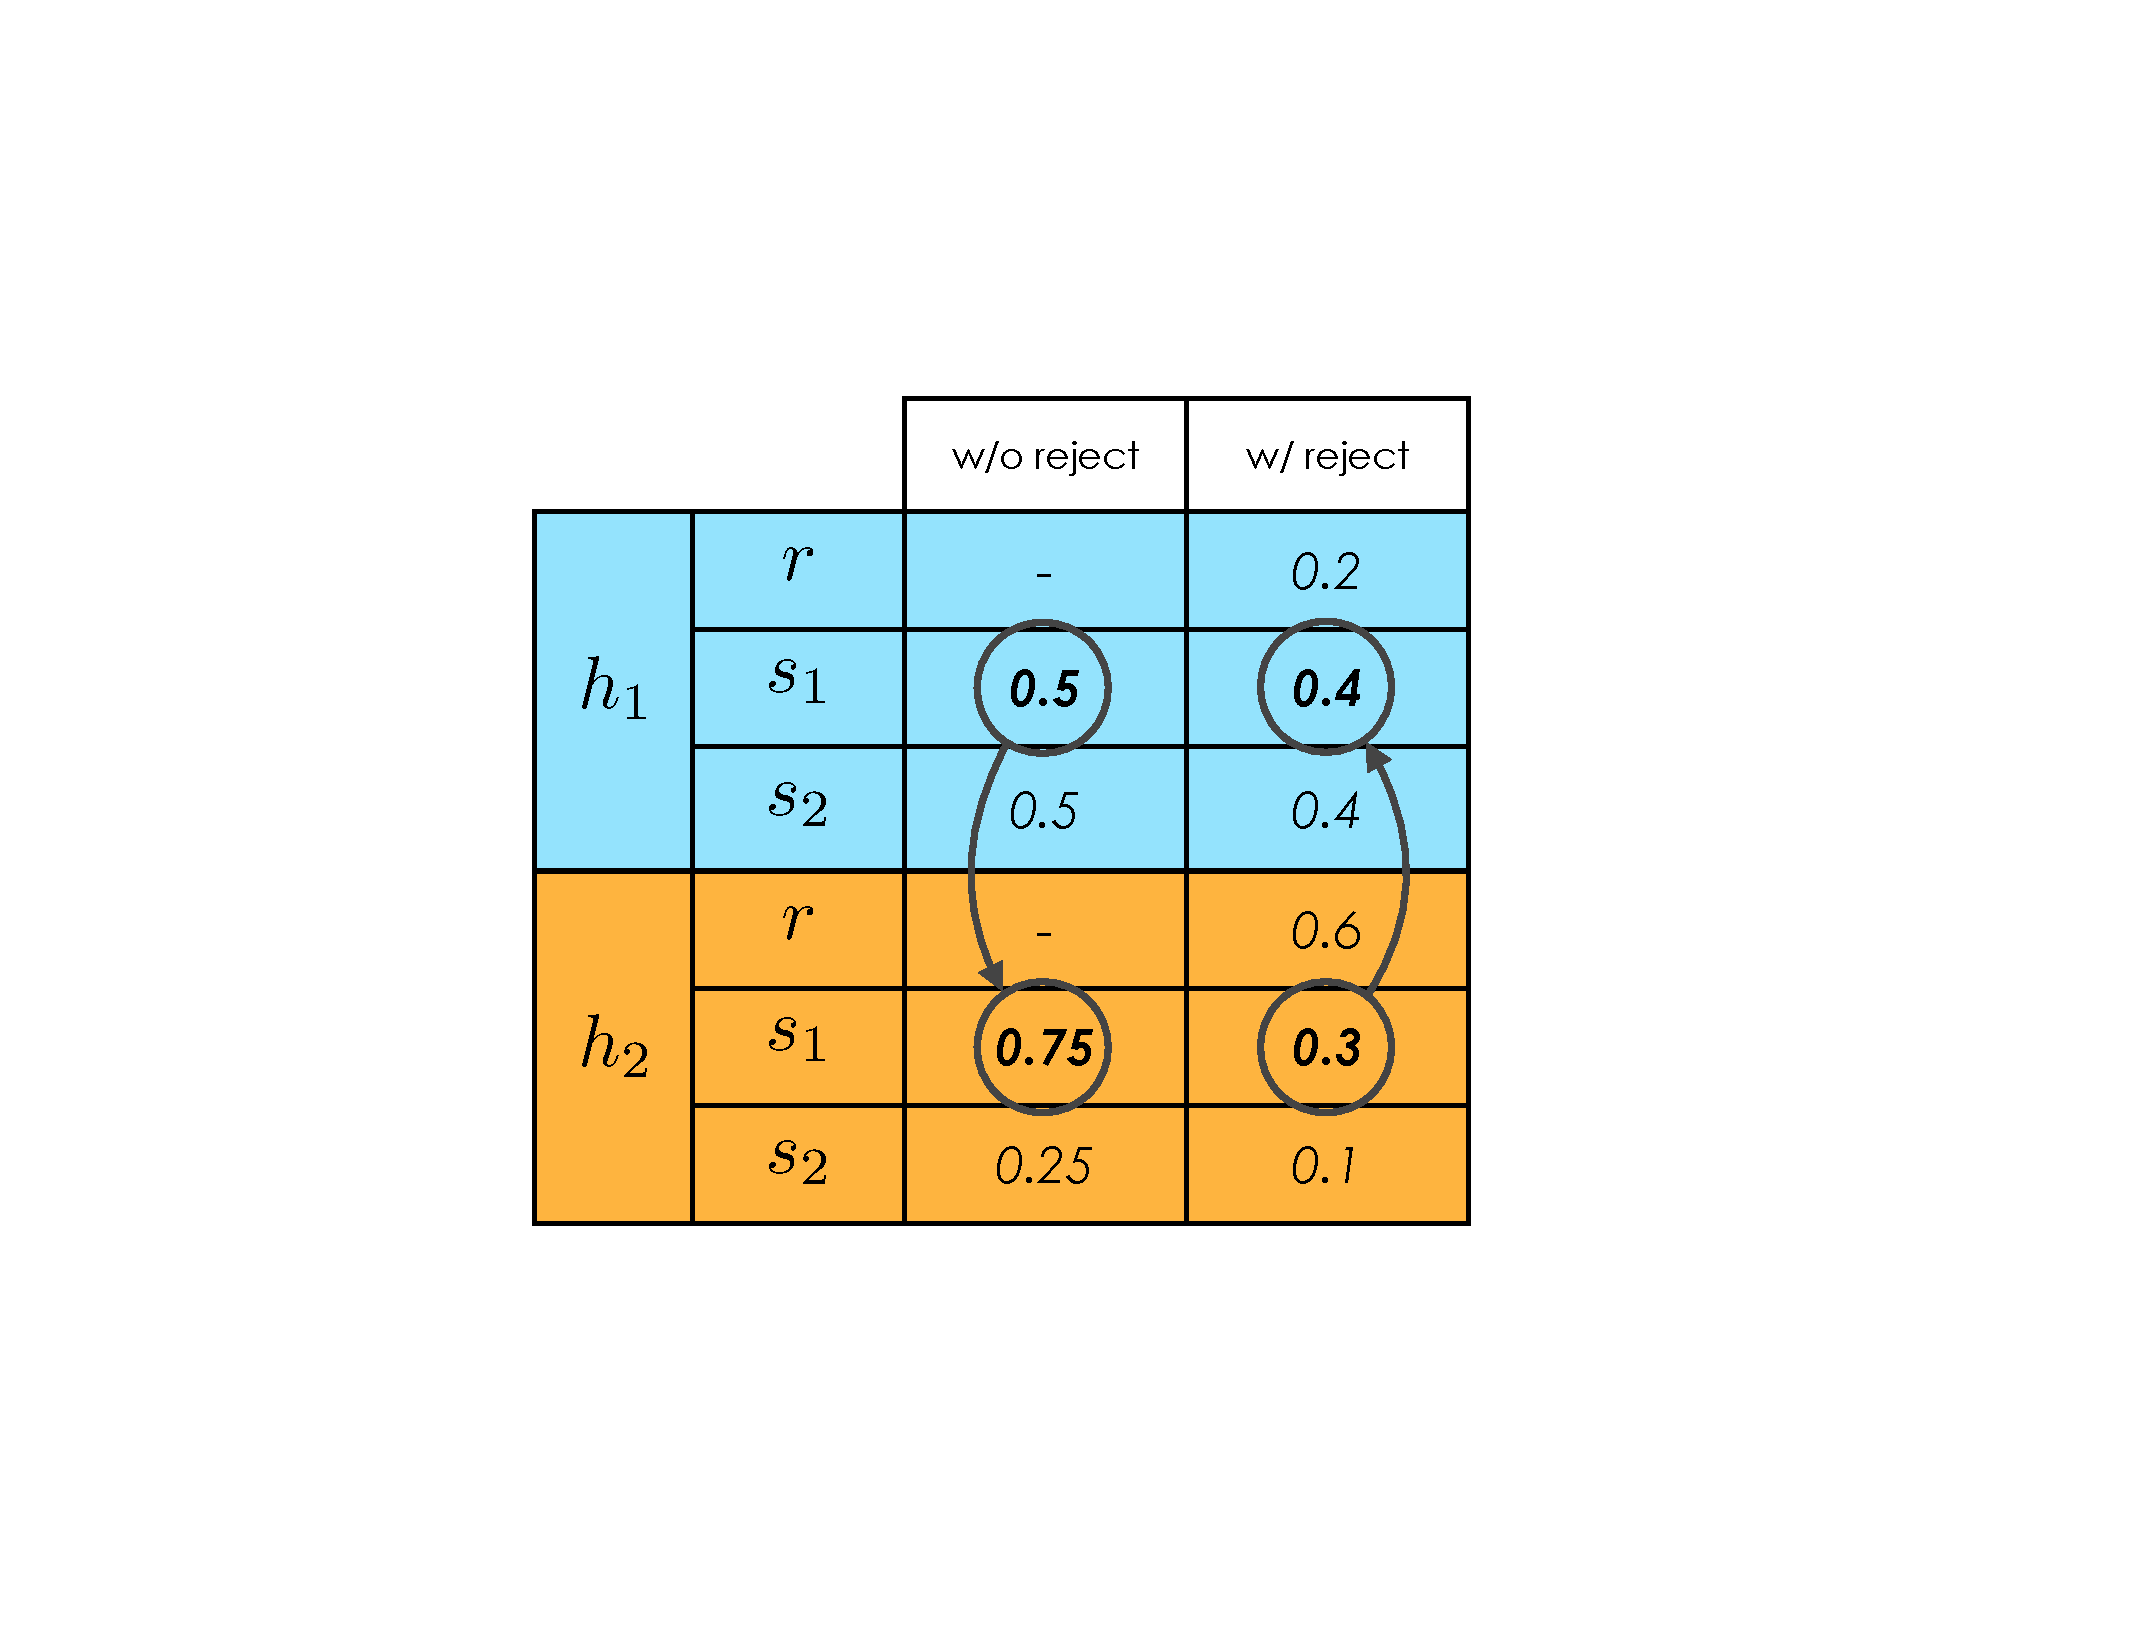
\includegraphics[width=0.6\linewidth]{figures/reject_vs_no_reject.pdf}
\caption{
Example of a case where modeling the reject option results in vastly different recommendation behavior.
Consider surfer $s_1$'s perspective: without modeling the reject option, $h_2$ looks more likely to accept $s_1$.
When modeling the reject option, however, the probabilities change and $h_1$ is now more likely to accept $s_1$, due to the ability to model how picky $h_2$ actually is.}
\label{fig:reject_vs_no_reject}
\end{figure}

\begin{eqnarray}
p(s_k | h_n, S_n) &=& \frac{\exp(\theta^T \Phi(s_k,h_n))}{\sum_{j \in S_n} \exp(\theta^T \Phi(s_j,h_n)) + \exp(r + r_{h_n})} \\
p(\text{reject} | h_n, S_n) &=& \frac{\exp(r+r_{h_n})}{\sum_{j \in S_n} \exp(\theta^T \Phi(s_j,h_n)) + \exp(r + r_{h_n})}
\end{eqnarray}
Note that $\Phi(s_k,h_n)$ also implicitly depends on the couchrequest (e.g. date, whether the host is already booked, etc.).

To have hostspecific parameters we would replace $\theta$ by $\theta + \theta_h$. 

Further, we want to add regularization for $\theta, \theta_h, r_{h_n}$.

Error (negative log likelihood)
\begin{eqnarray}
E(\theta, r, r_{h_n}) &=& - \log p(\{s_k\} | \{h_n\}, \{S_n\})\\
&=& - \log [ \prod_{n=1}^N \prod_{k=1}^K p(s_k | h_n, S_n)^{t_{nk}}]\\
&=&  - \sum_{n=1}^N \sum_{k=1}^K t_{nk} \log p(s_k | h_n, S_n)
\end{eqnarray}

To derive the gradient descent update steps we will take derivatives of $E(\theta, r, r_{h_n})$ wrt. $\theta, r, r_{h_n}$. Because we will do stochastic gradient descent we will basically ignore the sum over $n$ in the end (over different ``competitor sets $S_n$'') and just choose one at random. Note that here, we can just sample uniformly from all sets or sample a host first, and given that host, sample on of his sets. The latter will achieve that all hosts have the sample influence on the learning but we will have to discuss/test whether we actually want that.

We generally have:
\begin{eqnarray}
\frac{d}{d \theta} E(\theta, r, r_{h_n}) &=& - \sum_{n=1}^N \sum_{k=1}^K t_{nk} \frac{d}{d \theta}  \log p(s_k | h_n, S_n) \\
&=& - \sum_{n=1}^N \sum_{k=1}^K t_{nk} \frac{1}{p(s_k | h_n, S_n)} \frac{d}{d \theta} p(s_k | h_n, S_n)
\end{eqnarray}

Now we look at the individual derivatives of $p(s_k | h_n, S_n)$ and $p(\text{reject} | h_n, S_n)$.

1. Case: Some surfer $s_k$ gets chosen (no reject):
\begin{eqnarray}
\frac{d}{d \theta} p(s_k | h_n, S_n) = \frac{d}{d \theta} \frac{\exp(\theta^T \Phi(s_k,h_n))}{\sum_{j \in S_n} \exp(\theta^T \Phi(s_j,h_n)) + \exp(r + r_{h_n})} \\
= \frac{\Phi(s_k,h_n) [\sum_{j \in S_n} \exp(\theta^T \Phi(s_j,h_n)) + \exp(r + r_{h_n})]}{\sum_{j \in S_n} \exp(\theta^T \Phi(s_j,h_n)) + \exp(r + r_{h_n})} \\
- \frac{\exp(\theta^T \Phi(s_k,h_n)) [\sum_{j \in S_n} \Phi(s_j,h_n) \exp(\theta^T \Phi(s_j,h_n))]}{\sum_{j \in S_n} \exp(\theta^T \Phi(s_j,h_n)) + \exp(r + r_{h_n})}\\
= \Phi(s_k,h_n) p(s_k | h_n, S_n) - p(s_k | h_n, S_n) \frac{\sum_{j \in S_n} \Phi(s_j,h_n) \exp(\theta^T \Phi(s_j,h_n))}{\sum_{j \in S_n} \exp(\theta^T \Phi(s_j,h_n)) + \exp(r + r_{h_n})}\\
= p(s_k | h_n, S_n) (\Phi(s_k,h_n) - \sum_{j \in S_n} w_{jn} \Phi(s_j,h_n))
\end{eqnarray}
where $w_{jn}=\frac{\exp(\theta^T \Phi(s_j,h_n))}{\sum_{j \in S_n} \exp(\theta^T \Phi(s_j,h_n)) + \exp(r + r_{h_n})}$.

Thus, we get:
\begin{eqnarray}
\frac{d}{d \theta} E(\theta, r, r_{h_n}) = - \sum_{n=1}^N \sum_{k=1}^K t_{nk} \frac{1}{p(s_k | h_n, S_n)} \frac{d}{d \theta} p(s_k | h_n, S_n)\\
= - \sum_{n=1}^N \sum_{k=1}^K t_{nk} (\Phi(s_k,h_n) - \sum_{j \in S_n} w_{jn} \Phi(s_j,h_n)) \\
= \sum_{n=1}^N (\sum_{j \in S_n} w_{jn} \Phi(s_j,h_n) - \Phi(s_{k^*},h_n))
\end{eqnarray}
where $s_{k^*}$ is the surfer that got accepted from the competitor set $S_n$.

Similarly, taking the derivative wrt. $r$ ($r_{h_n}$ should be exactly the same) we obtain:
\begin{eqnarray}
\frac{d}{d r} p(s_k | h_n, S_n) = -  p(s_k | h_n, S_n)  \frac{\exp(r + r_{h_n})}{\sum_{j \in S_n} \exp(\theta^T \Phi(s_j,h_n)) + \exp(r + r_{h_n})}
\end{eqnarray}
Thus, we get:
\begin{eqnarray}
\frac{d}{d r} E(\theta, r, r_{h_n}) = - \sum_{n=1}^N \sum_{k=1}^K t_{nk} \frac{1}{p(s_k | h_n, S_n)} \frac{d}{d r} p(s_k | h_n, S_n)\\
= \sum_{n=1}^N \sum_{k=1}^K t_{nk} \frac{\exp(r + r_{h_n})}{\sum_{j \in S_n} \exp(\theta^T \Phi(s_j,h_n)) + \exp(r + r_{h_n})} \\
= \sum_{n=1}^N \frac{\exp(r + r_{h_n})}{\sum_{j \in S_n} \exp(\theta^T \Phi(s_j,h_n)) + \exp(r + r_{h_n})}
\end{eqnarray}



2. Case: No surfer gets chosen (reject):
\begin{eqnarray}
\frac{d}{d \theta} p(\text{reject} | h_n, S_n) = \frac{d}{d \theta} \frac{\exp(r+r_{h_n})}{\sum_{j \in S_n} \exp(\theta^T \Phi(s_j,h_n)) + \exp(r + r_{h_n})}\\
= - p(\text{reject} | h_n, S_n) \frac{\sum_{j \in S_n} \Phi(s_j,h_n) \exp(\theta^T \Phi(s_j,h_n))}{\sum_{j \in S_n} \exp(\theta^T \Phi(s_j,h_n)) + \exp(r + r_{h_n})} \\
= - p(\text{reject} | h_n, S_n) \sum_{j \in S_n} w_{jn} \Phi(s_j,h_n)
\end{eqnarray}
Thus, we get:
\begin{eqnarray}
\frac{d}{d \theta} E(\theta, r, r_{h_n}) = - \sum_{n=1}^N \sum_{k=1}^K t_{nk} \frac{1}{p(\text{reject} | h_n, S_n)} \frac{d}{d \theta} p(\text{reject} | h_n, S_n)\\
= \sum_{n=1}^N (\sum_{j \in S_n} w_{jn} \Phi(s_j,h_n))
\end{eqnarray}



Again, taking the derivative wrt. $r$ ($r_{h_n}$ should be exactly the same) we obtain:
\begin{eqnarray}
\frac{d}{d r} p(\text{reject} | h_n, S_n) = p(\text{reject} | h_n, S_n) - p(\text{reject} | h_n, S_n)^2\\
= p(\text{reject} | h_n, S_n) (1 - p(\text{reject} | h_n, S_n))\\
\end{eqnarray}
Thus, we get:
\begin{eqnarray}
\frac{d}{d r} E(\theta, r, r_{h_n}) = - \sum_{n=1}^N \sum_{k=1}^K t_{nk} \frac{1}{p(\text{reject} | h_n, S_n)} \frac{d}{d \theta} p(\text{reject} | h_n, S_n)\\
= \sum_{n=1}^N (p(\text{reject} | h_n, S_n)-1)
\end{eqnarray}


\paragraph{The final update equations}

Finally, for stochastic gradient descent the following update equations hold. We simply sample a host $h_n$ and competitor set $S_n$. Note that the following equations do not contain regularization, yet (although trivial).

1. Case: Some surfer $s_{k^*}$ gets chosen (no reject):
\begin{eqnarray}
\theta \leftarrow \theta - \eta (\sum_{j \in S_n} w_{jn} \Phi(s_j,h_n) - \Phi(s_{k^*},h_n))\\
r \leftarrow r - \eta \frac{\exp(r + r_{h_n})}{\sum_{j \in S_n} \exp(\theta^T \Phi(s_j,h_n)) + \exp(r + r_{h_n})}
\end{eqnarray}
where, again, $w_{jn}=\frac{\exp(\theta^T \Phi(s_j,h_n))}{\sum_{j \in S_n} \exp(\theta^T \Phi(s_j,h_n)) + \exp(r + r_{h_n})}$.

2. Case: No surfer gets chosen (reject):
\begin{eqnarray}
\theta \leftarrow \theta - \eta (\sum_{j \in S_n} w_{jn} \Phi(s_j,h_n))\\
r \leftarrow r - \eta (p(\text{reject} | h_n, S_n)-1)
\end{eqnarray}

For $l_2$-regularization, e.g. of $\theta$, just add $- \eta \lambda \theta$ to the update equation.